\section{Dobór parametrów lambda lokalnych regulatorów DMC}
\label{lab:zad6}

Złożoność rozmycia algorytmów DMC znacząco utrudnia intuicyjne dobieranie nastaw regulatorów.
Metoda polega na wielu próbach osiągnięcia lepszego wyniku co w 
przypadku rzeczywistego obiektu o stosunkowo dużej inercji jest wyjątkowo czasochłonne.


\subsection{Wyniki eksperymentów}
\label{lab:zad6:eksperymenty}

\begin{figure}[H] 
   \centering
   % This file was created by matlab2tikz.
%
\definecolor{mycolor1}{rgb}{0.00000,0.44700,0.74100}%
\definecolor{mycolor2}{rgb}{0.85000,0.32500,0.09800}%
%
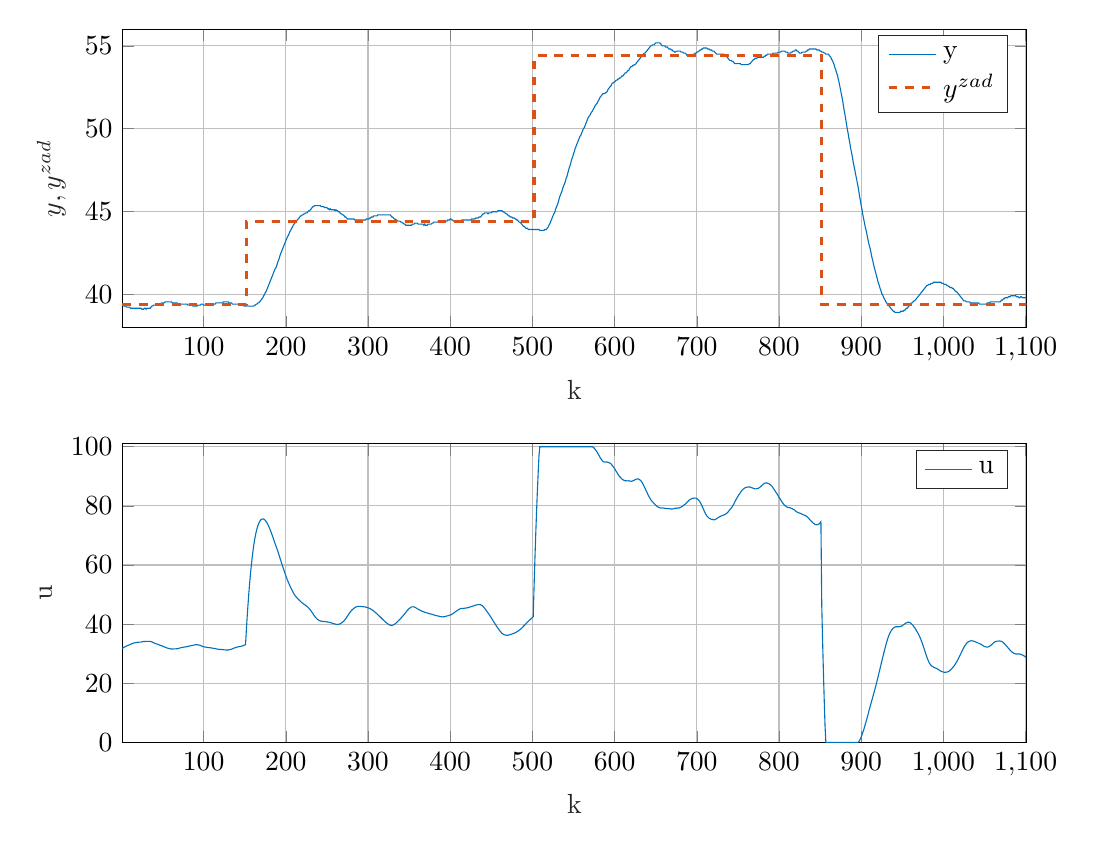
\begin{tikzpicture}

\begin{axis}[%
width=4.521in,
height=1.493in,
at={(0.758in,2.554in)},
scale only axis,
xmin=1,
xmax=1101,
xlabel style={font=\color{white!15!black}},
xlabel={k},
ymin=38,
ymax=56,
ylabel style={font=\color{white!15!black}},
ylabel={$\text{y, y}^{\text{zad}}$},
axis background/.style={fill=white},
xmajorgrids,
ymajorgrids,
legend style={legend cell align=left, align=left, draw=white!15!black}
]
\addplot [color=mycolor1]
  table[row sep=crcr]{%
1	39.37\\
2	39.37\\
3	39.31\\
4	39.31\\
5	39.31\\
6	39.25\\
7	39.25\\
8	39.25\\
9	39.25\\
10	39.25\\
11	39.18\\
12	39.18\\
13	39.18\\
14	39.18\\
15	39.18\\
16	39.18\\
17	39.18\\
18	39.18\\
19	39.18\\
20	39.18\\
21	39.18\\
22	39.18\\
23	39.18\\
24	39.18\\
25	39.12\\
26	39.12\\
27	39.12\\
28	39.18\\
29	39.18\\
30	39.12\\
31	39.18\\
32	39.18\\
33	39.18\\
34	39.18\\
35	39.18\\
36	39.25\\
37	39.31\\
38	39.31\\
39	39.37\\
40	39.37\\
41	39.37\\
42	39.37\\
43	39.37\\
44	39.37\\
45	39.43\\
46	39.43\\
47	39.43\\
48	39.43\\
49	39.5\\
50	39.5\\
51	39.5\\
52	39.5\\
53	39.56\\
54	39.56\\
55	39.56\\
56	39.56\\
57	39.56\\
58	39.56\\
59	39.56\\
60	39.56\\
61	39.56\\
62	39.5\\
63	39.5\\
64	39.5\\
65	39.5\\
66	39.5\\
67	39.5\\
68	39.5\\
69	39.43\\
70	39.43\\
71	39.43\\
72	39.43\\
73	39.43\\
74	39.43\\
75	39.43\\
76	39.43\\
77	39.43\\
78	39.43\\
79	39.43\\
80	39.43\\
81	39.37\\
82	39.37\\
83	39.37\\
84	39.37\\
85	39.37\\
86	39.37\\
87	39.31\\
88	39.31\\
89	39.31\\
90	39.31\\
91	39.31\\
92	39.31\\
93	39.37\\
94	39.37\\
95	39.37\\
96	39.37\\
97	39.43\\
98	39.43\\
99	39.43\\
100	39.37\\
101	39.37\\
102	39.37\\
103	39.37\\
104	39.37\\
105	39.37\\
106	39.37\\
107	39.37\\
108	39.37\\
109	39.37\\
110	39.43\\
111	39.43\\
112	39.43\\
113	39.43\\
114	39.43\\
115	39.5\\
116	39.5\\
117	39.5\\
118	39.5\\
119	39.5\\
120	39.5\\
121	39.5\\
122	39.5\\
123	39.5\\
124	39.56\\
125	39.56\\
126	39.56\\
127	39.56\\
128	39.56\\
129	39.56\\
130	39.56\\
131	39.5\\
132	39.5\\
133	39.5\\
134	39.5\\
135	39.43\\
136	39.43\\
137	39.43\\
138	39.43\\
139	39.43\\
140	39.43\\
141	39.43\\
142	39.43\\
143	39.43\\
144	39.43\\
145	39.43\\
146	39.43\\
147	39.37\\
148	39.37\\
149	39.31\\
150	39.31\\
151	39.31\\
152	39.31\\
153	39.37\\
154	39.31\\
155	39.31\\
156	39.31\\
157	39.31\\
158	39.31\\
159	39.31\\
160	39.31\\
161	39.31\\
162	39.37\\
163	39.37\\
164	39.43\\
165	39.43\\
166	39.5\\
167	39.5\\
168	39.56\\
169	39.62\\
170	39.68\\
171	39.75\\
172	39.81\\
173	39.93\\
174	40\\
175	40.12\\
176	40.18\\
177	40.31\\
178	40.43\\
179	40.56\\
180	40.68\\
181	40.81\\
182	40.93\\
183	41.06\\
184	41.18\\
185	41.31\\
186	41.43\\
187	41.56\\
188	41.62\\
189	41.75\\
190	41.93\\
191	42.06\\
192	42.18\\
193	42.37\\
194	42.5\\
195	42.62\\
196	42.75\\
197	42.87\\
198	43\\
199	43.12\\
200	43.25\\
201	43.37\\
202	43.5\\
203	43.56\\
204	43.68\\
205	43.81\\
206	43.87\\
207	44\\
208	44.06\\
209	44.18\\
210	44.25\\
211	44.31\\
212	44.37\\
213	44.43\\
214	44.5\\
215	44.56\\
216	44.62\\
217	44.68\\
218	44.75\\
219	44.75\\
220	44.81\\
221	44.81\\
222	44.87\\
223	44.87\\
224	44.93\\
225	44.93\\
226	44.93\\
227	45\\
228	45.06\\
229	45.06\\
230	45.12\\
231	45.18\\
232	45.25\\
233	45.31\\
234	45.31\\
235	45.37\\
236	45.37\\
237	45.37\\
238	45.37\\
239	45.37\\
240	45.37\\
241	45.37\\
242	45.37\\
243	45.31\\
244	45.31\\
245	45.31\\
246	45.31\\
247	45.25\\
248	45.25\\
249	45.25\\
250	45.25\\
251	45.18\\
252	45.18\\
253	45.12\\
254	45.18\\
255	45.12\\
256	45.12\\
257	45.12\\
258	45.12\\
259	45.12\\
260	45.06\\
261	45.12\\
262	45.06\\
263	45.06\\
264	45\\
265	45\\
266	44.93\\
267	44.87\\
268	44.87\\
269	44.81\\
270	44.81\\
271	44.75\\
272	44.68\\
273	44.68\\
274	44.62\\
275	44.56\\
276	44.56\\
277	44.56\\
278	44.56\\
279	44.56\\
280	44.56\\
281	44.56\\
282	44.56\\
283	44.56\\
284	44.5\\
285	44.5\\
286	44.5\\
287	44.5\\
288	44.5\\
289	44.5\\
290	44.5\\
291	44.5\\
292	44.5\\
293	44.5\\
294	44.5\\
295	44.5\\
296	44.5\\
297	44.5\\
298	44.56\\
299	44.56\\
300	44.56\\
301	44.56\\
302	44.62\\
303	44.62\\
304	44.68\\
305	44.68\\
306	44.68\\
307	44.75\\
308	44.75\\
309	44.75\\
310	44.75\\
311	44.75\\
312	44.81\\
313	44.81\\
314	44.81\\
315	44.81\\
316	44.81\\
317	44.81\\
318	44.81\\
319	44.81\\
320	44.81\\
321	44.81\\
322	44.81\\
323	44.81\\
324	44.81\\
325	44.81\\
326	44.81\\
327	44.81\\
328	44.75\\
329	44.68\\
330	44.68\\
331	44.62\\
332	44.56\\
333	44.56\\
334	44.5\\
335	44.5\\
336	44.43\\
337	44.43\\
338	44.43\\
339	44.43\\
340	44.37\\
341	44.37\\
342	44.31\\
343	44.31\\
344	44.25\\
345	44.25\\
346	44.18\\
347	44.18\\
348	44.18\\
349	44.18\\
350	44.18\\
351	44.18\\
352	44.18\\
353	44.18\\
354	44.25\\
355	44.25\\
356	44.25\\
357	44.31\\
358	44.31\\
359	44.31\\
360	44.31\\
361	44.25\\
362	44.25\\
363	44.25\\
364	44.25\\
365	44.25\\
366	44.25\\
367	44.25\\
368	44.18\\
369	44.25\\
370	44.18\\
371	44.18\\
372	44.18\\
373	44.25\\
374	44.25\\
375	44.25\\
376	44.25\\
377	44.25\\
378	44.31\\
379	44.31\\
380	44.37\\
381	44.37\\
382	44.37\\
383	44.37\\
384	44.37\\
385	44.37\\
386	44.43\\
387	44.43\\
388	44.43\\
389	44.43\\
390	44.43\\
391	44.43\\
392	44.43\\
393	44.43\\
394	44.43\\
395	44.43\\
396	44.43\\
397	44.5\\
398	44.5\\
399	44.5\\
400	44.56\\
401	44.56\\
402	44.5\\
403	44.5\\
404	44.43\\
405	44.43\\
406	44.43\\
407	44.43\\
408	44.43\\
409	44.43\\
410	44.37\\
411	44.37\\
412	44.43\\
413	44.43\\
414	44.5\\
415	44.5\\
416	44.5\\
417	44.5\\
418	44.5\\
419	44.5\\
420	44.5\\
421	44.5\\
422	44.5\\
423	44.5\\
424	44.5\\
425	44.5\\
426	44.56\\
427	44.56\\
428	44.56\\
429	44.56\\
430	44.56\\
431	44.62\\
432	44.62\\
433	44.62\\
434	44.62\\
435	44.68\\
436	44.68\\
437	44.68\\
438	44.75\\
439	44.81\\
440	44.87\\
441	44.87\\
442	44.93\\
443	44.93\\
444	44.93\\
445	44.93\\
446	44.87\\
447	44.93\\
448	44.93\\
449	44.93\\
450	44.93\\
451	45\\
452	45\\
453	45\\
454	45\\
455	45\\
456	45\\
457	45\\
458	45.06\\
459	45.06\\
460	45.06\\
461	45.06\\
462	45.06\\
463	45.06\\
464	45\\
465	45\\
466	44.93\\
467	44.93\\
468	44.87\\
469	44.87\\
470	44.81\\
471	44.75\\
472	44.75\\
473	44.68\\
474	44.68\\
475	44.68\\
476	44.62\\
477	44.62\\
478	44.62\\
479	44.56\\
480	44.56\\
481	44.5\\
482	44.5\\
483	44.43\\
484	44.37\\
485	44.37\\
486	44.31\\
487	44.25\\
488	44.18\\
489	44.12\\
490	44.12\\
491	44.06\\
492	44\\
493	44\\
494	44\\
495	43.93\\
496	43.93\\
497	43.93\\
498	43.93\\
499	43.93\\
500	43.93\\
501	43.93\\
502	43.93\\
503	43.93\\
504	43.93\\
505	43.93\\
506	43.93\\
507	43.93\\
508	43.93\\
509	43.87\\
510	43.87\\
511	43.87\\
512	43.87\\
513	43.87\\
514	43.87\\
515	43.93\\
516	43.93\\
517	43.93\\
518	44\\
519	44.06\\
520	44.18\\
521	44.25\\
522	44.37\\
523	44.5\\
524	44.62\\
525	44.75\\
526	44.87\\
527	44.93\\
528	45.12\\
529	45.25\\
530	45.37\\
531	45.5\\
532	45.68\\
533	45.87\\
534	46\\
535	46.12\\
536	46.25\\
537	46.43\\
538	46.56\\
539	46.68\\
540	46.81\\
541	47\\
542	47.12\\
543	47.31\\
544	47.5\\
545	47.68\\
546	47.81\\
547	48\\
548	48.18\\
549	48.31\\
550	48.5\\
551	48.62\\
552	48.81\\
553	48.93\\
554	49.06\\
555	49.18\\
556	49.31\\
557	49.43\\
558	49.56\\
559	49.62\\
560	49.75\\
561	49.87\\
562	50\\
563	50.06\\
564	50.18\\
565	50.31\\
566	50.43\\
567	50.56\\
568	50.68\\
569	50.75\\
570	50.81\\
571	50.93\\
572	51\\
573	51.06\\
574	51.18\\
575	51.25\\
576	51.37\\
577	51.43\\
578	51.5\\
579	51.56\\
580	51.68\\
581	51.75\\
582	51.87\\
583	51.93\\
584	52\\
585	52.06\\
586	52.12\\
587	52.12\\
588	52.12\\
589	52.18\\
590	52.18\\
591	52.25\\
592	52.37\\
593	52.43\\
594	52.5\\
595	52.56\\
596	52.62\\
597	52.75\\
598	52.75\\
599	52.81\\
600	52.81\\
601	52.87\\
602	52.93\\
603	52.93\\
604	53\\
605	53\\
606	53.06\\
607	53.06\\
608	53.12\\
609	53.18\\
610	53.18\\
611	53.25\\
612	53.31\\
613	53.37\\
614	53.37\\
615	53.43\\
616	53.5\\
617	53.5\\
618	53.62\\
619	53.68\\
620	53.75\\
621	53.75\\
622	53.81\\
623	53.81\\
624	53.87\\
625	53.87\\
626	53.93\\
627	54\\
628	54.06\\
629	54.12\\
630	54.18\\
631	54.25\\
632	54.31\\
633	54.37\\
634	54.43\\
635	54.5\\
636	54.56\\
637	54.56\\
638	54.62\\
639	54.68\\
640	54.75\\
641	54.81\\
642	54.87\\
643	54.93\\
644	55\\
645	55\\
646	55.06\\
647	55.06\\
648	55.06\\
649	55.12\\
650	55.18\\
651	55.18\\
652	55.18\\
653	55.18\\
654	55.18\\
655	55.18\\
656	55.12\\
657	55.06\\
658	55\\
659	55\\
660	55\\
661	55\\
662	54.93\\
663	54.93\\
664	54.93\\
665	54.87\\
666	54.81\\
667	54.81\\
668	54.81\\
669	54.75\\
670	54.75\\
671	54.68\\
672	54.68\\
673	54.62\\
674	54.62\\
675	54.68\\
676	54.68\\
677	54.68\\
678	54.68\\
679	54.68\\
680	54.68\\
681	54.62\\
682	54.62\\
683	54.62\\
684	54.56\\
685	54.56\\
686	54.56\\
687	54.5\\
688	54.43\\
689	54.43\\
690	54.37\\
691	54.37\\
692	54.37\\
693	54.43\\
694	54.43\\
695	54.43\\
696	54.5\\
697	54.5\\
698	54.56\\
699	54.56\\
700	54.62\\
701	54.62\\
702	54.68\\
703	54.68\\
704	54.75\\
705	54.75\\
706	54.81\\
707	54.81\\
708	54.87\\
709	54.87\\
710	54.87\\
711	54.87\\
712	54.87\\
713	54.81\\
714	54.81\\
715	54.81\\
716	54.75\\
717	54.75\\
718	54.75\\
719	54.68\\
720	54.68\\
721	54.68\\
722	54.62\\
723	54.56\\
724	54.5\\
725	54.5\\
726	54.5\\
727	54.5\\
728	54.5\\
729	54.5\\
730	54.5\\
731	54.5\\
732	54.5\\
733	54.5\\
734	54.43\\
735	54.43\\
736	54.37\\
737	54.31\\
738	54.25\\
739	54.18\\
740	54.12\\
741	54.12\\
742	54.12\\
743	54.06\\
744	54.06\\
745	54\\
746	53.93\\
747	53.93\\
748	53.93\\
749	53.93\\
750	53.93\\
751	53.93\\
752	53.93\\
753	53.93\\
754	53.87\\
755	53.87\\
756	53.87\\
757	53.87\\
758	53.87\\
759	53.87\\
760	53.87\\
761	53.87\\
762	53.87\\
763	53.87\\
764	53.93\\
765	53.93\\
766	54\\
767	54.06\\
768	54.12\\
769	54.18\\
770	54.18\\
771	54.25\\
772	54.25\\
773	54.25\\
774	54.31\\
775	54.31\\
776	54.31\\
777	54.31\\
778	54.31\\
779	54.31\\
780	54.31\\
781	54.31\\
782	54.37\\
783	54.37\\
784	54.43\\
785	54.43\\
786	54.5\\
787	54.5\\
788	54.5\\
789	54.5\\
790	54.5\\
791	54.5\\
792	54.5\\
793	54.56\\
794	54.56\\
795	54.56\\
796	54.56\\
797	54.56\\
798	54.56\\
799	54.62\\
800	54.62\\
801	54.62\\
802	54.62\\
803	54.68\\
804	54.68\\
805	54.68\\
806	54.68\\
807	54.68\\
808	54.62\\
809	54.62\\
810	54.62\\
811	54.56\\
812	54.56\\
813	54.56\\
814	54.56\\
815	54.62\\
816	54.62\\
817	54.68\\
818	54.68\\
819	54.68\\
820	54.75\\
821	54.75\\
822	54.68\\
823	54.68\\
824	54.62\\
825	54.56\\
826	54.56\\
827	54.56\\
828	54.62\\
829	54.62\\
830	54.62\\
831	54.62\\
832	54.62\\
833	54.68\\
834	54.68\\
835	54.75\\
836	54.75\\
837	54.81\\
838	54.81\\
839	54.81\\
840	54.81\\
841	54.81\\
842	54.81\\
843	54.81\\
844	54.81\\
845	54.81\\
846	54.75\\
847	54.75\\
848	54.75\\
849	54.75\\
850	54.68\\
851	54.68\\
852	54.62\\
853	54.62\\
854	54.62\\
855	54.56\\
856	54.56\\
857	54.5\\
858	54.5\\
859	54.5\\
860	54.5\\
861	54.43\\
862	54.37\\
863	54.31\\
864	54.18\\
865	54.12\\
866	54\\
867	53.87\\
868	53.68\\
869	53.56\\
870	53.37\\
871	53.25\\
872	53\\
873	52.81\\
874	52.56\\
875	52.31\\
876	52.06\\
877	51.81\\
878	51.5\\
879	51.18\\
880	50.93\\
881	50.62\\
882	50.31\\
883	50\\
884	49.75\\
885	49.43\\
886	49.18\\
887	48.87\\
888	48.62\\
889	48.37\\
890	48.06\\
891	47.81\\
892	47.56\\
893	47.31\\
894	47.06\\
895	46.81\\
896	46.56\\
897	46.25\\
898	45.93\\
899	45.68\\
900	45.37\\
901	45.12\\
902	44.81\\
903	44.56\\
904	44.31\\
905	44.06\\
906	43.87\\
907	43.62\\
908	43.37\\
909	43.12\\
910	42.93\\
911	42.75\\
912	42.5\\
913	42.25\\
914	42.06\\
915	41.81\\
916	41.62\\
917	41.43\\
918	41.25\\
919	41.06\\
920	40.87\\
921	40.68\\
922	40.56\\
923	40.37\\
924	40.25\\
925	40.06\\
926	40\\
927	39.87\\
928	39.75\\
929	39.68\\
930	39.56\\
931	39.5\\
932	39.43\\
933	39.37\\
934	39.31\\
935	39.25\\
936	39.18\\
937	39.12\\
938	39.06\\
939	39\\
940	39\\
941	38.93\\
942	38.93\\
943	38.93\\
944	38.93\\
945	38.93\\
946	38.93\\
947	38.93\\
948	39\\
949	39\\
950	39\\
951	39\\
952	39.06\\
953	39.06\\
954	39.12\\
955	39.18\\
956	39.18\\
957	39.25\\
958	39.31\\
959	39.37\\
960	39.43\\
961	39.5\\
962	39.5\\
963	39.56\\
964	39.62\\
965	39.62\\
966	39.68\\
967	39.75\\
968	39.81\\
969	39.87\\
970	39.93\\
971	40\\
972	40.06\\
973	40.12\\
974	40.18\\
975	40.25\\
976	40.31\\
977	40.37\\
978	40.43\\
979	40.5\\
980	40.56\\
981	40.56\\
982	40.62\\
983	40.62\\
984	40.62\\
985	40.68\\
986	40.68\\
987	40.68\\
988	40.75\\
989	40.75\\
990	40.75\\
991	40.75\\
992	40.75\\
993	40.75\\
994	40.75\\
995	40.75\\
996	40.75\\
997	40.75\\
998	40.68\\
999	40.68\\
1000	40.68\\
1001	40.62\\
1002	40.62\\
1003	40.62\\
1004	40.56\\
1005	40.56\\
1006	40.5\\
1007	40.5\\
1008	40.43\\
1009	40.43\\
1010	40.43\\
1011	40.37\\
1012	40.37\\
1013	40.31\\
1014	40.25\\
1015	40.18\\
1016	40.18\\
1017	40.12\\
1018	40.06\\
1019	40\\
1020	39.93\\
1021	39.87\\
1022	39.81\\
1023	39.75\\
1024	39.68\\
1025	39.62\\
1026	39.62\\
1027	39.62\\
1028	39.56\\
1029	39.56\\
1030	39.56\\
1031	39.56\\
1032	39.56\\
1033	39.5\\
1034	39.5\\
1035	39.5\\
1036	39.5\\
1037	39.5\\
1038	39.5\\
1039	39.5\\
1040	39.5\\
1041	39.5\\
1042	39.5\\
1043	39.5\\
1044	39.43\\
1045	39.43\\
1046	39.43\\
1047	39.43\\
1048	39.43\\
1049	39.43\\
1050	39.43\\
1051	39.43\\
1052	39.43\\
1053	39.5\\
1054	39.5\\
1055	39.5\\
1056	39.5\\
1057	39.56\\
1058	39.56\\
1059	39.56\\
1060	39.56\\
1061	39.56\\
1062	39.56\\
1063	39.56\\
1064	39.56\\
1065	39.56\\
1066	39.56\\
1067	39.56\\
1068	39.56\\
1069	39.56\\
1070	39.62\\
1071	39.68\\
1072	39.68\\
1073	39.75\\
1074	39.75\\
1075	39.81\\
1076	39.81\\
1077	39.81\\
1078	39.81\\
1079	39.87\\
1080	39.87\\
1081	39.87\\
1082	39.93\\
1083	39.93\\
1084	39.93\\
1085	39.93\\
1086	39.93\\
1087	39.93\\
1088	39.93\\
1089	39.87\\
1090	39.87\\
1091	39.87\\
1092	39.81\\
1093	39.81\\
1094	39.87\\
1095	39.87\\
1096	39.81\\
1097	39.81\\
1098	39.81\\
1099	39.81\\
1100	39.81\\
1101	39.81\\
};
\addlegendentry{y}

\addplot[const plot, color=mycolor2, dashed, line width=1.2pt] table[row sep=crcr] {%
1	39.4\\
2	39.4\\
3	39.4\\
4	39.4\\
5	39.4\\
6	39.4\\
7	39.4\\
8	39.4\\
9	39.4\\
10	39.4\\
11	39.4\\
12	39.4\\
13	39.4\\
14	39.4\\
15	39.4\\
16	39.4\\
17	39.4\\
18	39.4\\
19	39.4\\
20	39.4\\
21	39.4\\
22	39.4\\
23	39.4\\
24	39.4\\
25	39.4\\
26	39.4\\
27	39.4\\
28	39.4\\
29	39.4\\
30	39.4\\
31	39.4\\
32	39.4\\
33	39.4\\
34	39.4\\
35	39.4\\
36	39.4\\
37	39.4\\
38	39.4\\
39	39.4\\
40	39.4\\
41	39.4\\
42	39.4\\
43	39.4\\
44	39.4\\
45	39.4\\
46	39.4\\
47	39.4\\
48	39.4\\
49	39.4\\
50	39.4\\
51	39.4\\
52	39.4\\
53	39.4\\
54	39.4\\
55	39.4\\
56	39.4\\
57	39.4\\
58	39.4\\
59	39.4\\
60	39.4\\
61	39.4\\
62	39.4\\
63	39.4\\
64	39.4\\
65	39.4\\
66	39.4\\
67	39.4\\
68	39.4\\
69	39.4\\
70	39.4\\
71	39.4\\
72	39.4\\
73	39.4\\
74	39.4\\
75	39.4\\
76	39.4\\
77	39.4\\
78	39.4\\
79	39.4\\
80	39.4\\
81	39.4\\
82	39.4\\
83	39.4\\
84	39.4\\
85	39.4\\
86	39.4\\
87	39.4\\
88	39.4\\
89	39.4\\
90	39.4\\
91	39.4\\
92	39.4\\
93	39.4\\
94	39.4\\
95	39.4\\
96	39.4\\
97	39.4\\
98	39.4\\
99	39.4\\
100	39.4\\
101	39.4\\
102	39.4\\
103	39.4\\
104	39.4\\
105	39.4\\
106	39.4\\
107	39.4\\
108	39.4\\
109	39.4\\
110	39.4\\
111	39.4\\
112	39.4\\
113	39.4\\
114	39.4\\
115	39.4\\
116	39.4\\
117	39.4\\
118	39.4\\
119	39.4\\
120	39.4\\
121	39.4\\
122	39.4\\
123	39.4\\
124	39.4\\
125	39.4\\
126	39.4\\
127	39.4\\
128	39.4\\
129	39.4\\
130	39.4\\
131	39.4\\
132	39.4\\
133	39.4\\
134	39.4\\
135	39.4\\
136	39.4\\
137	39.4\\
138	39.4\\
139	39.4\\
140	39.4\\
141	39.4\\
142	39.4\\
143	39.4\\
144	39.4\\
145	39.4\\
146	39.4\\
147	39.4\\
148	39.4\\
149	39.4\\
150	39.4\\
151	39.4\\
152	44.4\\
153	44.4\\
154	44.4\\
155	44.4\\
156	44.4\\
157	44.4\\
158	44.4\\
159	44.4\\
160	44.4\\
161	44.4\\
162	44.4\\
163	44.4\\
164	44.4\\
165	44.4\\
166	44.4\\
167	44.4\\
168	44.4\\
169	44.4\\
170	44.4\\
171	44.4\\
172	44.4\\
173	44.4\\
174	44.4\\
175	44.4\\
176	44.4\\
177	44.4\\
178	44.4\\
179	44.4\\
180	44.4\\
181	44.4\\
182	44.4\\
183	44.4\\
184	44.4\\
185	44.4\\
186	44.4\\
187	44.4\\
188	44.4\\
189	44.4\\
190	44.4\\
191	44.4\\
192	44.4\\
193	44.4\\
194	44.4\\
195	44.4\\
196	44.4\\
197	44.4\\
198	44.4\\
199	44.4\\
200	44.4\\
201	44.4\\
202	44.4\\
203	44.4\\
204	44.4\\
205	44.4\\
206	44.4\\
207	44.4\\
208	44.4\\
209	44.4\\
210	44.4\\
211	44.4\\
212	44.4\\
213	44.4\\
214	44.4\\
215	44.4\\
216	44.4\\
217	44.4\\
218	44.4\\
219	44.4\\
220	44.4\\
221	44.4\\
222	44.4\\
223	44.4\\
224	44.4\\
225	44.4\\
226	44.4\\
227	44.4\\
228	44.4\\
229	44.4\\
230	44.4\\
231	44.4\\
232	44.4\\
233	44.4\\
234	44.4\\
235	44.4\\
236	44.4\\
237	44.4\\
238	44.4\\
239	44.4\\
240	44.4\\
241	44.4\\
242	44.4\\
243	44.4\\
244	44.4\\
245	44.4\\
246	44.4\\
247	44.4\\
248	44.4\\
249	44.4\\
250	44.4\\
251	44.4\\
252	44.4\\
253	44.4\\
254	44.4\\
255	44.4\\
256	44.4\\
257	44.4\\
258	44.4\\
259	44.4\\
260	44.4\\
261	44.4\\
262	44.4\\
263	44.4\\
264	44.4\\
265	44.4\\
266	44.4\\
267	44.4\\
268	44.4\\
269	44.4\\
270	44.4\\
271	44.4\\
272	44.4\\
273	44.4\\
274	44.4\\
275	44.4\\
276	44.4\\
277	44.4\\
278	44.4\\
279	44.4\\
280	44.4\\
281	44.4\\
282	44.4\\
283	44.4\\
284	44.4\\
285	44.4\\
286	44.4\\
287	44.4\\
288	44.4\\
289	44.4\\
290	44.4\\
291	44.4\\
292	44.4\\
293	44.4\\
294	44.4\\
295	44.4\\
296	44.4\\
297	44.4\\
298	44.4\\
299	44.4\\
300	44.4\\
301	44.4\\
302	44.4\\
303	44.4\\
304	44.4\\
305	44.4\\
306	44.4\\
307	44.4\\
308	44.4\\
309	44.4\\
310	44.4\\
311	44.4\\
312	44.4\\
313	44.4\\
314	44.4\\
315	44.4\\
316	44.4\\
317	44.4\\
318	44.4\\
319	44.4\\
320	44.4\\
321	44.4\\
322	44.4\\
323	44.4\\
324	44.4\\
325	44.4\\
326	44.4\\
327	44.4\\
328	44.4\\
329	44.4\\
330	44.4\\
331	44.4\\
332	44.4\\
333	44.4\\
334	44.4\\
335	44.4\\
336	44.4\\
337	44.4\\
338	44.4\\
339	44.4\\
340	44.4\\
341	44.4\\
342	44.4\\
343	44.4\\
344	44.4\\
345	44.4\\
346	44.4\\
347	44.4\\
348	44.4\\
349	44.4\\
350	44.4\\
351	44.4\\
352	44.4\\
353	44.4\\
354	44.4\\
355	44.4\\
356	44.4\\
357	44.4\\
358	44.4\\
359	44.4\\
360	44.4\\
361	44.4\\
362	44.4\\
363	44.4\\
364	44.4\\
365	44.4\\
366	44.4\\
367	44.4\\
368	44.4\\
369	44.4\\
370	44.4\\
371	44.4\\
372	44.4\\
373	44.4\\
374	44.4\\
375	44.4\\
376	44.4\\
377	44.4\\
378	44.4\\
379	44.4\\
380	44.4\\
381	44.4\\
382	44.4\\
383	44.4\\
384	44.4\\
385	44.4\\
386	44.4\\
387	44.4\\
388	44.4\\
389	44.4\\
390	44.4\\
391	44.4\\
392	44.4\\
393	44.4\\
394	44.4\\
395	44.4\\
396	44.4\\
397	44.4\\
398	44.4\\
399	44.4\\
400	44.4\\
401	44.4\\
402	44.4\\
403	44.4\\
404	44.4\\
405	44.4\\
406	44.4\\
407	44.4\\
408	44.4\\
409	44.4\\
410	44.4\\
411	44.4\\
412	44.4\\
413	44.4\\
414	44.4\\
415	44.4\\
416	44.4\\
417	44.4\\
418	44.4\\
419	44.4\\
420	44.4\\
421	44.4\\
422	44.4\\
423	44.4\\
424	44.4\\
425	44.4\\
426	44.4\\
427	44.4\\
428	44.4\\
429	44.4\\
430	44.4\\
431	44.4\\
432	44.4\\
433	44.4\\
434	44.4\\
435	44.4\\
436	44.4\\
437	44.4\\
438	44.4\\
439	44.4\\
440	44.4\\
441	44.4\\
442	44.4\\
443	44.4\\
444	44.4\\
445	44.4\\
446	44.4\\
447	44.4\\
448	44.4\\
449	44.4\\
450	44.4\\
451	44.4\\
452	44.4\\
453	44.4\\
454	44.4\\
455	44.4\\
456	44.4\\
457	44.4\\
458	44.4\\
459	44.4\\
460	44.4\\
461	44.4\\
462	44.4\\
463	44.4\\
464	44.4\\
465	44.4\\
466	44.4\\
467	44.4\\
468	44.4\\
469	44.4\\
470	44.4\\
471	44.4\\
472	44.4\\
473	44.4\\
474	44.4\\
475	44.4\\
476	44.4\\
477	44.4\\
478	44.4\\
479	44.4\\
480	44.4\\
481	44.4\\
482	44.4\\
483	44.4\\
484	44.4\\
485	44.4\\
486	44.4\\
487	44.4\\
488	44.4\\
489	44.4\\
490	44.4\\
491	44.4\\
492	44.4\\
493	44.4\\
494	44.4\\
495	44.4\\
496	44.4\\
497	44.4\\
498	44.4\\
499	44.4\\
500	44.4\\
501	44.4\\
502	54.4\\
503	54.4\\
504	54.4\\
505	54.4\\
506	54.4\\
507	54.4\\
508	54.4\\
509	54.4\\
510	54.4\\
511	54.4\\
512	54.4\\
513	54.4\\
514	54.4\\
515	54.4\\
516	54.4\\
517	54.4\\
518	54.4\\
519	54.4\\
520	54.4\\
521	54.4\\
522	54.4\\
523	54.4\\
524	54.4\\
525	54.4\\
526	54.4\\
527	54.4\\
528	54.4\\
529	54.4\\
530	54.4\\
531	54.4\\
532	54.4\\
533	54.4\\
534	54.4\\
535	54.4\\
536	54.4\\
537	54.4\\
538	54.4\\
539	54.4\\
540	54.4\\
541	54.4\\
542	54.4\\
543	54.4\\
544	54.4\\
545	54.4\\
546	54.4\\
547	54.4\\
548	54.4\\
549	54.4\\
550	54.4\\
551	54.4\\
552	54.4\\
553	54.4\\
554	54.4\\
555	54.4\\
556	54.4\\
557	54.4\\
558	54.4\\
559	54.4\\
560	54.4\\
561	54.4\\
562	54.4\\
563	54.4\\
564	54.4\\
565	54.4\\
566	54.4\\
567	54.4\\
568	54.4\\
569	54.4\\
570	54.4\\
571	54.4\\
572	54.4\\
573	54.4\\
574	54.4\\
575	54.4\\
576	54.4\\
577	54.4\\
578	54.4\\
579	54.4\\
580	54.4\\
581	54.4\\
582	54.4\\
583	54.4\\
584	54.4\\
585	54.4\\
586	54.4\\
587	54.4\\
588	54.4\\
589	54.4\\
590	54.4\\
591	54.4\\
592	54.4\\
593	54.4\\
594	54.4\\
595	54.4\\
596	54.4\\
597	54.4\\
598	54.4\\
599	54.4\\
600	54.4\\
601	54.4\\
602	54.4\\
603	54.4\\
604	54.4\\
605	54.4\\
606	54.4\\
607	54.4\\
608	54.4\\
609	54.4\\
610	54.4\\
611	54.4\\
612	54.4\\
613	54.4\\
614	54.4\\
615	54.4\\
616	54.4\\
617	54.4\\
618	54.4\\
619	54.4\\
620	54.4\\
621	54.4\\
622	54.4\\
623	54.4\\
624	54.4\\
625	54.4\\
626	54.4\\
627	54.4\\
628	54.4\\
629	54.4\\
630	54.4\\
631	54.4\\
632	54.4\\
633	54.4\\
634	54.4\\
635	54.4\\
636	54.4\\
637	54.4\\
638	54.4\\
639	54.4\\
640	54.4\\
641	54.4\\
642	54.4\\
643	54.4\\
644	54.4\\
645	54.4\\
646	54.4\\
647	54.4\\
648	54.4\\
649	54.4\\
650	54.4\\
651	54.4\\
652	54.4\\
653	54.4\\
654	54.4\\
655	54.4\\
656	54.4\\
657	54.4\\
658	54.4\\
659	54.4\\
660	54.4\\
661	54.4\\
662	54.4\\
663	54.4\\
664	54.4\\
665	54.4\\
666	54.4\\
667	54.4\\
668	54.4\\
669	54.4\\
670	54.4\\
671	54.4\\
672	54.4\\
673	54.4\\
674	54.4\\
675	54.4\\
676	54.4\\
677	54.4\\
678	54.4\\
679	54.4\\
680	54.4\\
681	54.4\\
682	54.4\\
683	54.4\\
684	54.4\\
685	54.4\\
686	54.4\\
687	54.4\\
688	54.4\\
689	54.4\\
690	54.4\\
691	54.4\\
692	54.4\\
693	54.4\\
694	54.4\\
695	54.4\\
696	54.4\\
697	54.4\\
698	54.4\\
699	54.4\\
700	54.4\\
701	54.4\\
702	54.4\\
703	54.4\\
704	54.4\\
705	54.4\\
706	54.4\\
707	54.4\\
708	54.4\\
709	54.4\\
710	54.4\\
711	54.4\\
712	54.4\\
713	54.4\\
714	54.4\\
715	54.4\\
716	54.4\\
717	54.4\\
718	54.4\\
719	54.4\\
720	54.4\\
721	54.4\\
722	54.4\\
723	54.4\\
724	54.4\\
725	54.4\\
726	54.4\\
727	54.4\\
728	54.4\\
729	54.4\\
730	54.4\\
731	54.4\\
732	54.4\\
733	54.4\\
734	54.4\\
735	54.4\\
736	54.4\\
737	54.4\\
738	54.4\\
739	54.4\\
740	54.4\\
741	54.4\\
742	54.4\\
743	54.4\\
744	54.4\\
745	54.4\\
746	54.4\\
747	54.4\\
748	54.4\\
749	54.4\\
750	54.4\\
751	54.4\\
752	54.4\\
753	54.4\\
754	54.4\\
755	54.4\\
756	54.4\\
757	54.4\\
758	54.4\\
759	54.4\\
760	54.4\\
761	54.4\\
762	54.4\\
763	54.4\\
764	54.4\\
765	54.4\\
766	54.4\\
767	54.4\\
768	54.4\\
769	54.4\\
770	54.4\\
771	54.4\\
772	54.4\\
773	54.4\\
774	54.4\\
775	54.4\\
776	54.4\\
777	54.4\\
778	54.4\\
779	54.4\\
780	54.4\\
781	54.4\\
782	54.4\\
783	54.4\\
784	54.4\\
785	54.4\\
786	54.4\\
787	54.4\\
788	54.4\\
789	54.4\\
790	54.4\\
791	54.4\\
792	54.4\\
793	54.4\\
794	54.4\\
795	54.4\\
796	54.4\\
797	54.4\\
798	54.4\\
799	54.4\\
800	54.4\\
801	54.4\\
802	54.4\\
803	54.4\\
804	54.4\\
805	54.4\\
806	54.4\\
807	54.4\\
808	54.4\\
809	54.4\\
810	54.4\\
811	54.4\\
812	54.4\\
813	54.4\\
814	54.4\\
815	54.4\\
816	54.4\\
817	54.4\\
818	54.4\\
819	54.4\\
820	54.4\\
821	54.4\\
822	54.4\\
823	54.4\\
824	54.4\\
825	54.4\\
826	54.4\\
827	54.4\\
828	54.4\\
829	54.4\\
830	54.4\\
831	54.4\\
832	54.4\\
833	54.4\\
834	54.4\\
835	54.4\\
836	54.4\\
837	54.4\\
838	54.4\\
839	54.4\\
840	54.4\\
841	54.4\\
842	54.4\\
843	54.4\\
844	54.4\\
845	54.4\\
846	54.4\\
847	54.4\\
848	54.4\\
849	54.4\\
850	54.4\\
851	54.4\\
852	39.4\\
853	39.4\\
854	39.4\\
855	39.4\\
856	39.4\\
857	39.4\\
858	39.4\\
859	39.4\\
860	39.4\\
861	39.4\\
862	39.4\\
863	39.4\\
864	39.4\\
865	39.4\\
866	39.4\\
867	39.4\\
868	39.4\\
869	39.4\\
870	39.4\\
871	39.4\\
872	39.4\\
873	39.4\\
874	39.4\\
875	39.4\\
876	39.4\\
877	39.4\\
878	39.4\\
879	39.4\\
880	39.4\\
881	39.4\\
882	39.4\\
883	39.4\\
884	39.4\\
885	39.4\\
886	39.4\\
887	39.4\\
888	39.4\\
889	39.4\\
890	39.4\\
891	39.4\\
892	39.4\\
893	39.4\\
894	39.4\\
895	39.4\\
896	39.4\\
897	39.4\\
898	39.4\\
899	39.4\\
900	39.4\\
901	39.4\\
902	39.4\\
903	39.4\\
904	39.4\\
905	39.4\\
906	39.4\\
907	39.4\\
908	39.4\\
909	39.4\\
910	39.4\\
911	39.4\\
912	39.4\\
913	39.4\\
914	39.4\\
915	39.4\\
916	39.4\\
917	39.4\\
918	39.4\\
919	39.4\\
920	39.4\\
921	39.4\\
922	39.4\\
923	39.4\\
924	39.4\\
925	39.4\\
926	39.4\\
927	39.4\\
928	39.4\\
929	39.4\\
930	39.4\\
931	39.4\\
932	39.4\\
933	39.4\\
934	39.4\\
935	39.4\\
936	39.4\\
937	39.4\\
938	39.4\\
939	39.4\\
940	39.4\\
941	39.4\\
942	39.4\\
943	39.4\\
944	39.4\\
945	39.4\\
946	39.4\\
947	39.4\\
948	39.4\\
949	39.4\\
950	39.4\\
951	39.4\\
952	39.4\\
953	39.4\\
954	39.4\\
955	39.4\\
956	39.4\\
957	39.4\\
958	39.4\\
959	39.4\\
960	39.4\\
961	39.4\\
962	39.4\\
963	39.4\\
964	39.4\\
965	39.4\\
966	39.4\\
967	39.4\\
968	39.4\\
969	39.4\\
970	39.4\\
971	39.4\\
972	39.4\\
973	39.4\\
974	39.4\\
975	39.4\\
976	39.4\\
977	39.4\\
978	39.4\\
979	39.4\\
980	39.4\\
981	39.4\\
982	39.4\\
983	39.4\\
984	39.4\\
985	39.4\\
986	39.4\\
987	39.4\\
988	39.4\\
989	39.4\\
990	39.4\\
991	39.4\\
992	39.4\\
993	39.4\\
994	39.4\\
995	39.4\\
996	39.4\\
997	39.4\\
998	39.4\\
999	39.4\\
1000	39.4\\
1001	39.4\\
1002	39.4\\
1003	39.4\\
1004	39.4\\
1005	39.4\\
1006	39.4\\
1007	39.4\\
1008	39.4\\
1009	39.4\\
1010	39.4\\
1011	39.4\\
1012	39.4\\
1013	39.4\\
1014	39.4\\
1015	39.4\\
1016	39.4\\
1017	39.4\\
1018	39.4\\
1019	39.4\\
1020	39.4\\
1021	39.4\\
1022	39.4\\
1023	39.4\\
1024	39.4\\
1025	39.4\\
1026	39.4\\
1027	39.4\\
1028	39.4\\
1029	39.4\\
1030	39.4\\
1031	39.4\\
1032	39.4\\
1033	39.4\\
1034	39.4\\
1035	39.4\\
1036	39.4\\
1037	39.4\\
1038	39.4\\
1039	39.4\\
1040	39.4\\
1041	39.4\\
1042	39.4\\
1043	39.4\\
1044	39.4\\
1045	39.4\\
1046	39.4\\
1047	39.4\\
1048	39.4\\
1049	39.4\\
1050	39.4\\
1051	39.4\\
1052	39.4\\
1053	39.4\\
1054	39.4\\
1055	39.4\\
1056	39.4\\
1057	39.4\\
1058	39.4\\
1059	39.4\\
1060	39.4\\
1061	39.4\\
1062	39.4\\
1063	39.4\\
1064	39.4\\
1065	39.4\\
1066	39.4\\
1067	39.4\\
1068	39.4\\
1069	39.4\\
1070	39.4\\
1071	39.4\\
1072	39.4\\
1073	39.4\\
1074	39.4\\
1075	39.4\\
1076	39.4\\
1077	39.4\\
1078	39.4\\
1079	39.4\\
1080	39.4\\
1081	39.4\\
1082	39.4\\
1083	39.4\\
1084	39.4\\
1085	39.4\\
1086	39.4\\
1087	39.4\\
1088	39.4\\
1089	39.4\\
1090	39.4\\
1091	39.4\\
1092	39.4\\
1093	39.4\\
1094	39.4\\
1095	39.4\\
1096	39.4\\
1097	39.4\\
1098	39.4\\
1099	39.4\\
1100	39.4\\
1101	39.4\\
};
\addlegendentry{$\text{y}^{\text{zad}}$}

\end{axis}

\begin{axis}[%
width=4.521in,
height=1.493in,
at={(0.758in,0.481in)},
scale only axis,
xmin=1,
xmax=1101,
xlabel style={font=\color{white!15!black}},
xlabel={k},
ymin=0,
ymax=101,
ylabel style={font=\color{white!15!black}},
ylabel={u},
axis background/.style={fill=white},
xmajorgrids,
ymajorgrids,
legend style={legend cell align=left, align=left, draw=white!15!black}
]
\addplot [color=mycolor1]
  table[row sep=crcr]{%
1	31.8406493913083\\
2	31.9674620223148\\
3	32.1353184660954\\
4	32.2822474326452\\
5	32.4091873093112\\
6	32.5758651832947\\
7	32.7202443418278\\
8	32.8450115520087\\
9	32.9513485228528\\
10	33.0427004214435\\
11	33.186959391447\\
12	33.3141986267407\\
13	33.4260484987239\\
14	33.5234786647029\\
15	33.6076725033527\\
16	33.6790512255844\\
17	33.7396652566074\\
18	33.7902918236051\\
19	33.83197536127\\
20	33.8659229409421\\
21	33.8940550228029\\
22	33.9163446007608\\
23	33.9337269105258\\
24	33.947730706226\\
25	34.0166877173841\\
26	34.0792081346659\\
27	34.136185361924\\
28	34.1307561817489\\
29	34.1263270029439\\
30	34.1798781086751\\
31	34.1730884369293\\
32	34.168737045048\\
33	34.1670105767316\\
34	34.1675375545883\\
35	34.1694405927526\\
36	34.1062020520377\\
37	33.9922808577433\\
38	33.8896596100744\\
39	33.7409118244593\\
40	33.6069741605061\\
41	33.4870841910985\\
42	33.3818188565951\\
43	33.2900808297454\\
44	33.2115908306228\\
45	33.0864326220699\\
46	32.977677419992\\
47	32.8845104401406\\
48	32.8053792510979\\
49	32.6717022518146\\
50	32.5541179025983\\
51	32.451404107001\\
52	32.3622316518461\\
53	32.2278960954291\\
54	32.1082908311027\\
55	32.0028607704592\\
56	31.9096451853683\\
57	31.8280993988702\\
58	31.7561931079976\\
59	31.6918465807033\\
60	31.6340971397958\\
61	31.584017825677\\
62	31.5979777350396\\
63	31.6132747856786\\
64	31.6290475019021\\
65	31.6448135885757\\
66	31.6611683925228\\
67	31.6771424700664\\
68	31.6929789867363\\
69	31.7757313437021\\
70	31.8538567137709\\
71	31.9262624015394\\
72	31.9947963888073\\
73	32.0593099141088\\
74	32.1197132494352\\
75	32.174777691476\\
76	32.2270691189232\\
77	32.2751834636329\\
78	32.3190048358489\\
79	32.3585024991567\\
80	32.3933255627279\\
81	32.4808104494654\\
82	32.5589516152692\\
83	32.6273424423029\\
84	32.6859338375326\\
85	32.7337933164414\\
86	32.7711038886212\\
87	32.8562508468775\\
88	32.9268007110354\\
89	32.9824588739065\\
90	33.0236126316607\\
91	33.0517645922902\\
92	33.0677145420414\\
93	33.0135415893214\\
94	32.9531914036772\\
95	32.8873732283371\\
96	32.8172261591126\\
97	32.6868144632325\\
98	32.5592981379696\\
99	32.4346521722202\\
100	32.3723268415466\\
101	32.3117510615856\\
102	32.2539536950242\\
103	32.1997451776726\\
104	32.1500731591459\\
105	32.1062071875061\\
106	32.0682695572345\\
107	32.0369047486377\\
108	32.0127531874279\\
109	31.9948674461405\\
110	31.9259171909173\\
111	31.868454728555\\
112	31.8226057158446\\
113	31.7870770586176\\
114	31.7617711517485\\
115	31.6783725992836\\
116	31.6085101495603\\
117	31.5511982062388\\
118	31.5052254866577\\
119	31.4698576660929\\
120	31.4445729411371\\
121	31.4279198514882\\
122	31.4196462500614\\
123	31.4185696470988\\
124	31.3662423274948\\
125	31.3247364709581\\
126	31.2946988129421\\
127	31.2741156807754\\
128	31.2621171428318\\
129	31.2580163882035\\
130	31.2618288570309\\
131	31.3296319300972\\
132	31.3973151121269\\
133	31.4635884677149\\
134	31.5286515285721\\
135	31.659196837649\\
136	31.7824650401839\\
137	31.8964106796996\\
138	32.0016392082963\\
139	32.0975414397856\\
140	32.1843478789227\\
141	32.2623882130629\\
142	32.3309036047267\\
143	32.3896250214132\\
144	32.4405150414061\\
145	32.4854804843987\\
146	32.5243882177033\\
147	32.6152414494879\\
148	32.6963449804293\\
149	32.8273676957074\\
150	32.9474479375981\\
151	33.0564302581091\\
152	37.9547801171565\\
153	42.4094849117205\\
154	46.5550080177519\\
155	50.3460490734497\\
156	53.7993811294878\\
157	56.9303629572773\\
158	59.7679251596671\\
159	62.3255465387842\\
160	64.6193397514847\\
161	66.6622365428233\\
162	68.410834955214\\
163	69.9516208779235\\
164	71.2389874892125\\
165	72.3595616750287\\
166	73.2657404636181\\
167	74.035859384658\\
168	74.6301147304478\\
169	75.0686383014012\\
170	75.3716182106535\\
171	75.5459111205261\\
172	75.615835308892\\
173	75.5368659121451\\
174	75.3754448790949\\
175	75.0940045344225\\
176	74.7638906011809\\
177	74.3258823652265\\
178	73.8154351914793\\
179	73.2326023341759\\
180	72.594782385024\\
181	71.9017071542515\\
182	71.1808534211524\\
183	70.4268540456483\\
184	69.6553409989998\\
185	68.8606119916857\\
186	68.0547572676473\\
187	67.2314812229938\\
188	66.4626757526552\\
189	65.678764163718\\
190	64.8459381246985\\
191	64.0185505596779\\
192	63.1941991428213\\
193	62.3074064920656\\
194	61.4216518127711\\
195	60.5468063679846\\
196	59.6873090489138\\
197	58.850387347639\\
198	58.0252397445518\\
199	57.2221947200037\\
200	56.4283598412505\\
201	55.6630700594513\\
202	54.9147728122663\\
203	54.2470633134278\\
204	53.5940365145591\\
205	52.9427031021312\\
206	52.3592056569667\\
207	51.7687824106693\\
208	51.2373352877797\\
209	50.7007769020536\\
210	50.2188545269185\\
211	49.7919270072444\\
212	49.4130440926032\\
213	49.0765299218696\\
214	48.7662028427529\\
215	48.4743122622152\\
216	48.196553727313\\
217	47.9295929031991\\
218	47.6489308554866\\
219	47.4242366486846\\
220	47.1914002482449\\
221	46.9955687606899\\
222	46.7757583022533\\
223	46.5798535890169\\
224	46.3498617901693\\
225	46.1343072577066\\
226	45.9362246765232\\
227	45.6776533220964\\
228	45.3760206621944\\
229	45.0833484622384\\
230	44.7458359868162\\
231	44.369896513474\\
232	43.9561350620125\\
233	43.5211958226823\\
234	43.1277689708831\\
235	42.7187833153164\\
236	42.3591330992156\\
237	42.0483315929469\\
238	41.7732389040036\\
239	41.547656249851\\
240	41.3565266356659\\
241	41.2027504676417\\
242	41.0735021975233\\
243	41.0275837096046\\
244	40.9912571827283\\
245	40.9549101386004\\
246	40.9104268611478\\
247	40.9095547550988\\
248	40.884640611736\\
249	40.8319604956006\\
250	40.7609860887103\\
251	40.7345952424808\\
252	40.6792969036543\\
253	40.6505413996311\\
254	40.5399610424695\\
255	40.4650565883538\\
256	40.3777128128104\\
257	40.286919016131\\
258	40.1896371075993\\
259	40.0939294958872\\
260	40.0528432846173\\
261	39.9553067542085\\
262	39.9294347336682\\
263	39.9081740012034\\
264	39.9559140156228\\
265	40.0040803622716\\
266	40.1259126801736\\
267	40.3010508706196\\
268	40.4744106401693\\
269	40.6967761275401\\
270	40.9154256917961\\
271	41.1934393773283\\
272	41.5404696136028\\
273	41.8879749713565\\
274	42.2839226605801\\
275	42.7306021210065\\
276	43.1565106551196\\
277	43.5671347797984\\
278	43.954790697152\\
279	44.3130115783113\\
280	44.6359999636557\\
281	44.9205211463877\\
282	45.1753341193664\\
283	45.3835047179982\\
284	45.6018977166314\\
285	45.7683380106723\\
286	45.8853328450534\\
287	45.9651680801102\\
288	46.0081107854886\\
289	46.0273583359519\\
290	46.0225100279246\\
291	46.0067529990959\\
292	45.9785268693362\\
293	45.9494102941471\\
294	45.9157531142669\\
295	45.8760442291468\\
296	45.8399598954982\\
297	45.8038362134645\\
298	45.7066311414859\\
299	45.6187729577724\\
300	45.5360194954096\\
301	45.4550617046877\\
302	45.3138467684058\\
303	45.1844356898511\\
304	45.0042115973422\\
305	44.8308887587852\\
306	44.659923490149\\
307	44.4209927521866\\
308	44.1838711287367\\
309	43.9448977690667\\
310	43.7147551713235\\
311	43.489984601644\\
312	43.2099767020048\\
313	42.9344849254677\\
314	42.6604171364703\\
315	42.3873568598016\\
316	42.1143210138599\\
317	41.8417477906211\\
318	41.5690427865733\\
319	41.2967984244422\\
320	41.0380400934583\\
321	40.7927049331066\\
322	40.5604278382306\\
323	40.3412357647096\\
324	40.1347329550606\\
325	39.9527755021824\\
326	39.7924304083485\\
327	39.6522471579694\\
328	39.5864389675003\\
329	39.6122701078476\\
330	39.6514207440142\\
331	39.758154177989\\
332	39.9351289774382\\
333	40.1149166800788\\
334	40.3616040619333\\
335	40.606283391546\\
336	40.9110635995042\\
337	41.1978154757218\\
338	41.4749918646109\\
339	41.7368008914121\\
340	42.0377505595369\\
341	42.3261480051827\\
342	42.6552879984191\\
343	42.9595504719395\\
344	43.3061201857946\\
345	43.6292754136816\\
346	44.0054351266889\\
347	44.3588783239665\\
348	44.6860583540593\\
349	44.985904208533\\
350	45.2564011685831\\
351	45.4849430761195\\
352	45.6732257352312\\
353	45.8224269873223\\
354	45.8675386591741\\
355	45.8718930990166\\
356	45.8388007558032\\
357	45.7141785537069\\
358	45.5643574303563\\
359	45.3924976643534\\
360	45.2017898552538\\
361	45.0639283429932\\
362	44.9175047931793\\
363	44.7744473862223\\
364	44.6341044055712\\
365	44.4946252724798\\
366	44.3547052419593\\
367	44.213589532585\\
368	44.1367034296171\\
369	43.9965049053058\\
370	43.9297985842592\\
371	43.8621440642829\\
372	43.8067084178563\\
373	43.6934419401572\\
374	43.5926424548484\\
375	43.5127235472976\\
376	43.4519554016567\\
377	43.4069533933261\\
378	43.3189239981348\\
379	43.246558000286\\
380	43.1310132402049\\
381	43.0338708980058\\
382	42.9525764240615\\
383	42.8863522136393\\
384	42.8327783157784\\
385	42.791288213999\\
386	42.702016489447\\
387	42.6268872535336\\
388	42.5650203961587\\
389	42.515008033775\\
390	42.488922389257\\
391	42.4830485432957\\
392	42.4957553161155\\
393	42.5352464647682\\
394	42.5987142288531\\
395	42.68170310952\\
396	42.7808218324177\\
397	42.8396406205403\\
398	42.92447712905\\
399	43.0306263515091\\
400	43.0952464315987\\
401	43.1764049373567\\
402	43.3276378275926\\
403	43.482722009421\\
404	43.7060673176122\\
405	43.9224903109138\\
406	44.130679377743\\
407	44.3283477150893\\
408	44.51541032916\\
409	44.6905830136849\\
410	44.8972748406395\\
411	45.0753232300219\\
412	45.1832899702547\\
413	45.2830893568982\\
414	45.3076499606059\\
415	45.3296827522747\\
416	45.348651359414\\
417	45.3759342745417\\
418	45.4096539695623\\
419	45.4478557512415\\
420	45.4901296615267\\
421	45.5468287575132\\
422	45.6135557394892\\
423	45.6999477933076\\
424	45.8008915556616\\
425	45.9121249471931\\
426	45.9727182873402\\
427	46.0543073048159\\
428	46.1515343225241\\
429	46.2602378784219\\
430	46.376046376547\\
431	46.4369946308081\\
432	46.5012580881624\\
433	46.5659702944216\\
434	46.6272787605751\\
435	46.62506090527\\
436	46.6046846856683\\
437	46.5654421553264\\
438	46.4394778181389\\
439	46.241452091447\\
440	45.9647466853922\\
441	45.6731094612818\\
442	45.310946499522\\
443	44.9425282679891\\
444	44.558161283104\\
445	44.1616026873735\\
446	43.8149131126488\\
447	43.4016609363864\\
448	42.9892572995785\\
449	42.581090839811\\
450	42.1676705930857\\
451	41.6871794182769\\
452	41.2164260767014\\
453	40.7581415193519\\
454	40.3151973737455\\
455	39.8894965574629\\
456	39.4815127382165\\
457	39.0934921971336\\
458	38.666654326388\\
459	38.2634489789502\\
460	37.8839756477226\\
461	37.5269180784517\\
462	37.2030343014363\\
463	36.909154036469\\
464	36.6998836592241\\
465	36.5088964094563\\
466	36.4020765683152\\
467	36.303768268607\\
468	36.269544061537\\
469	36.2346981911057\\
470	36.2549732711905\\
471	36.3246236658577\\
472	36.3808049351677\\
473	36.4900579223176\\
474	36.5800861151329\\
475	36.6516318072616\\
476	36.7627464094968\\
477	36.864577937296\\
478	36.9563279164214\\
479	37.0966593444825\\
480	37.2232803107353\\
481	37.3953751069425\\
482	37.552050852121\\
483	37.7500745117306\\
484	37.9772664992493\\
485	38.1745771908139\\
486	38.4036468247696\\
487	38.6614336662555\\
488	38.9437883544691\\
489	39.2523493372091\\
490	39.5148468954368\\
491	39.8056218119974\\
492	40.1212139147309\\
493	40.4017427427582\\
494	40.6485239131757\\
495	40.9428362363674\\
496	41.2221818164431\\
497	41.4862982000987\\
498	41.7475774541022\\
499	42.0013581533904\\
500	42.258578037981\\
501	42.5262680646745\\
502	52.4004139731722\\
503	61.5251386240278\\
504	69.9293601545886\\
505	77.6424940085857\\
506	84.6943780864816\\
507	91.1158558013953\\
508	96.9623492361727\\
509	100\\
510	100\\
511	100\\
512	100\\
513	100\\
514	100\\
515	100\\
516	100\\
517	100\\
518	100\\
519	100\\
520	100\\
521	100\\
522	100\\
523	100\\
524	100\\
525	100\\
526	100\\
527	100\\
528	100\\
529	100\\
530	100\\
531	100\\
532	100\\
533	100\\
534	100\\
535	100\\
536	100\\
537	100\\
538	100\\
539	100\\
540	100\\
541	100\\
542	100\\
543	100\\
544	100\\
545	100\\
546	100\\
547	100\\
548	100\\
549	100\\
550	100\\
551	100\\
552	100\\
553	100\\
554	100\\
555	100\\
556	100\\
557	100\\
558	100\\
559	100\\
560	100\\
561	100\\
562	100\\
563	100\\
564	100\\
565	100\\
566	100\\
567	100\\
568	100\\
569	100\\
570	100\\
571	100\\
572	100\\
573	100\\
574	99.8092620852691\\
575	99.5811598248716\\
576	99.2348392531141\\
577	98.8853695998297\\
578	98.5043308659326\\
579	98.0872867038488\\
580	97.5514490784316\\
581	97.0734106186603\\
582	96.5233064174253\\
583	96.0764833206143\\
584	95.6557128951502\\
585	95.3018683828432\\
586	95.0123732689211\\
587	94.9031928083659\\
588	94.847180544264\\
589	94.798341944327\\
590	94.8550496226038\\
591	94.8541803700846\\
592	94.7193231761353\\
593	94.6511472425737\\
594	94.5213503257355\\
595	94.3565955660538\\
596	94.1341490702443\\
597	93.7041732777724\\
598	93.3968475209811\\
599	92.9579535113766\\
600	92.6147178534104\\
601	92.1553431894776\\
602	91.6524348355992\\
603	91.225745993372\\
604	90.7276976083913\\
605	90.3390572505835\\
606	89.9258361382802\\
607	89.6673133749723\\
608	89.3400849543712\\
609	89.0618477276034\\
610	88.9122349685844\\
611	88.7245409918141\\
612	88.6022934292835\\
613	88.4894600763535\\
614	88.5200338337495\\
615	88.4783674646695\\
616	88.445599257416\\
617	88.5225858096986\\
618	88.4388907618651\\
619	88.3804467314468\\
620	88.3143254513282\\
621	88.3942651483245\\
622	88.4295651498871\\
623	88.6031461534805\\
624	88.684590347069\\
625	88.8967790351616\\
626	89.0057479474648\\
627	89.0912139936301\\
628	89.1274197309328\\
629	89.0883263728964\\
630	88.9646356344086\\
631	88.7394673480705\\
632	88.4887853130491\\
633	88.1202109713253\\
634	87.6667772915954\\
635	87.109979115937\\
636	86.4991944906467\\
637	85.9957482920873\\
638	85.3946606517449\\
639	84.8028578112884\\
640	84.1766276939165\\
641	83.6198185780031\\
642	83.0781875216807\\
643	82.5978248359524\\
644	82.1108269968121\\
645	81.7513156838427\\
646	81.3666102204231\\
647	81.0923476425071\\
648	80.8511099281514\\
649	80.5591123308012\\
650	80.2429503169278\\
651	80.0067328402288\\
652	79.7884966086049\\
653	79.6273923227663\\
654	79.4755339694938\\
655	79.3344434116034\\
656	79.301765936391\\
657	79.300168277691\\
658	79.3314100842924\\
659	79.2752913967607\\
660	79.2279761918252\\
661	79.1519328466126\\
662	79.1894901847333\\
663	79.1303816865602\\
664	79.0479287299129\\
665	79.0606403654895\\
666	79.1040615763296\\
667	79.0485896109932\\
668	78.9557662492971\\
669	78.9536454033627\\
670	78.915308783646\\
671	79.0097660168271\\
672	79.0259715098783\\
673	79.1517511951592\\
674	79.2054200968795\\
675	79.1842773602032\\
676	79.233897498349\\
677	79.2788135040189\\
678	79.3064720865064\\
679	79.3792496997903\\
680	79.4554533967713\\
681	79.6464224255132\\
682	79.7993350882327\\
683	79.9336747612336\\
684	80.2168720985936\\
685	80.4314519478989\\
686	80.6178100320649\\
687	80.8803903306411\\
688	81.2268663299007\\
689	81.4644432505127\\
690	81.7729424844513\\
691	82.0224506588252\\
692	82.2335524279928\\
693	82.2996268400316\\
694	82.448144117224\\
695	82.576615151826\\
696	82.5877240506435\\
697	82.6705862601629\\
698	82.619848281855\\
699	82.6063027305298\\
700	82.4614314181676\\
701	82.3084507152249\\
702	81.9934288372156\\
703	81.7008436014552\\
704	81.2329878931055\\
705	80.7696128804367\\
706	80.1583557963992\\
707	79.5904443723199\\
708	78.9063467288986\\
709	78.3012973616808\\
710	77.7075732663894\\
711	77.1740101286998\\
712	76.6840593555911\\
713	76.4003148488447\\
714	76.1009413490144\\
715	75.8382412134786\\
716	75.7205968586297\\
717	75.558289797426\\
718	75.396404632001\\
719	75.4080398045296\\
720	75.3428958998356\\
721	75.2638823721941\\
722	75.3464974903062\\
723	75.4894498947289\\
724	75.685926954612\\
725	75.8620795807568\\
726	76.0379424346638\\
727	76.2026964614407\\
728	76.3663278490031\\
729	76.5134705542868\\
730	76.6400182019873\\
731	76.7555694857039\\
732	76.8507632981286\\
733	76.9227409855126\\
734	77.1132204840535\\
735	77.2170394677758\\
736	77.4214223491925\\
737	77.6633840331837\\
738	77.9378908844587\\
739	78.2647018666371\\
740	78.6570673106247\\
741	78.9777028635186\\
742	79.2883698464692\\
743	79.7508120478145\\
744	80.1508383280416\\
745	80.6636754073124\\
746	81.2393515524037\\
747	81.7693824394193\\
748	82.2806881305028\\
749	82.7800864667531\\
750	83.2505001868612\\
751	83.6847406018779\\
752	84.0901940464362\\
753	84.465508146271\\
754	84.911805266338\\
755	85.2406263861855\\
756	85.5274454152084\\
757	85.7745553125982\\
758	85.9870952561199\\
759	86.165490936169\\
760	86.2599685326654\\
761	86.3102916324785\\
762	86.3812997356141\\
763	86.4410654407113\\
764	86.3794253005134\\
765	86.3779114328024\\
766	86.2441869095896\\
767	86.1391417712215\\
768	86.0326007159321\\
769	85.9009160826131\\
770	85.8513309968971\\
771	85.7440815432099\\
772	85.7556029743652\\
773	85.8574101115103\\
774	85.8822358021903\\
775	85.9991591705365\\
776	86.1462079194963\\
777	86.3723810963719\\
778	86.6251197144297\\
779	86.88633826814\\
780	87.1472234416952\\
781	87.3970821003742\\
782	87.5232432016186\\
783	87.7056431678029\\
784	87.7477511972182\\
785	87.8208812771664\\
786	87.6800060934021\\
787	87.5740725356542\\
788	87.4330385556249\\
789	87.2632430075397\\
790	87.0193147821735\\
791	86.736267956911\\
792	86.4253742732635\\
793	85.9879166423477\\
794	85.5754009476538\\
795	85.1491671230885\\
796	84.7185832322891\\
797	84.2976121487265\\
798	83.9005045414652\\
799	83.4054733183714\\
800	82.9470764389032\\
801	82.509399025487\\
802	82.0999817738615\\
803	81.5993511747686\\
804	81.18818732142\\
805	80.8045193249632\\
806	80.4465902275149\\
807	80.1247462169711\\
808	79.9571962921233\\
809	79.7492705584192\\
810	79.5595511191672\\
811	79.4994733851126\\
812	79.4281961758293\\
813	79.374176288673\\
814	79.331648083635\\
815	79.1788471106507\\
816	79.0921791286862\\
817	78.8911617308407\\
818	78.7531557673242\\
819	78.6011265547877\\
820	78.2922908235745\\
821	78.0486717195666\\
822	77.9313012839317\\
823	77.7304630205139\\
824	77.6356228887555\\
825	77.5830637749836\\
826	77.4549507086657\\
827	77.3659385036902\\
828	77.1717584125335\\
829	77.0539932028479\\
830	76.9508827439412\\
831	76.8615375369103\\
832	76.788550230969\\
833	76.566290971261\\
834	76.398608342245\\
835	76.0840717091917\\
836	75.8448539861782\\
837	75.4951780503206\\
838	75.1717711176784\\
839	74.8907150372118\\
840	74.5846993025001\\
841	74.3394426109207\\
842	74.1143655853563\\
843	73.9065513292978\\
844	73.7117241045818\\
845	73.5863664107742\\
846	73.6548732750573\\
847	73.6924859422292\\
848	73.8165543321042\\
849	73.9657727915963\\
850	74.3239565284865\\
851	74.6850393682457\\
852	46.3900573949595\\
853	34.6786526526397\\
854	23.9882905492361\\
855	14.3774305179031\\
856	5.60536751969486\\
857	0\\
858	0\\
859	0\\
860	0\\
861	0\\
862	0\\
863	0\\
864	0\\
865	0\\
866	0\\
867	0\\
868	0\\
869	0\\
870	0\\
871	0\\
872	0\\
873	0\\
874	0\\
875	0\\
876	0\\
877	0\\
878	0\\
879	0\\
880	0\\
881	0\\
882	0\\
883	0\\
884	0\\
885	0\\
886	0\\
887	0\\
888	0\\
889	0\\
890	0\\
891	0\\
892	0\\
893	0\\
894	0\\
895	0\\
896	0.0103945609627043\\
897	0.231207682920246\\
898	0.655531628379457\\
899	1.17886683483071\\
900	1.85153522313833\\
901	2.56906350004022\\
902	3.38559591191103\\
903	4.25627674694114\\
904	5.17770498633178\\
905	6.14630465451481\\
906	7.09752022696554\\
907	8.09250492627006\\
908	9.14376335404889\\
909	10.2455306184317\\
910	11.2930017786343\\
911	12.2823351505925\\
912	13.2869126165933\\
913	14.3027790397805\\
914	15.2738998092984\\
915	16.298006042031\\
916	17.3171859730532\\
917	18.3472671020061\\
918	19.4109079505877\\
919	20.5024170406491\\
920	21.618056829883\\
921	22.7818471684469\\
922	23.9007954351597\\
923	25.0759832609866\\
924	26.2238081797011\\
925	27.4278164841224\\
926	28.5480688214985\\
927	29.6838347123244\\
928	30.8013569772459\\
929	31.8804330667029\\
930	32.9493162753221\\
931	33.9433221204608\\
932	34.853198011533\\
933	35.673720830932\\
934	36.395731944565\\
935	37.0241157593967\\
936	37.5555287403457\\
937	37.9888898878652\\
938	38.3685380743383\\
939	38.6631733505384\\
940	38.8563899786015\\
941	39.0147906594993\\
942	39.1080208710963\\
943	39.1378400582089\\
944	39.1371463918678\\
945	39.1245973892913\\
946	39.1408216698929\\
947	39.194139520357\\
948	39.2380544795183\\
949	39.3476416665899\\
950	39.4993277557694\\
951	39.6952711850188\\
952	39.87801139775\\
953	40.1097747018459\\
954	40.2964296833319\\
955	40.4477317770501\\
956	40.5906663078212\\
957	40.6461433231497\\
958	40.6385164151956\\
959	40.5460676213665\\
960	40.3899130666716\\
961	40.1528631639229\\
962	39.8828279926218\\
963	39.5581143598938\\
964	39.173486319338\\
965	38.8071792057017\\
966	38.3910799756438\\
967	37.9351286931853\\
968	37.4445183472201\\
969	36.9518679881498\\
970	36.4269914462797\\
971	35.8523953705552\\
972	35.2192393782253\\
973	34.523622304823\\
974	33.7868872331841\\
975	32.9859591896117\\
976	32.1532217110919\\
977	31.2862705044661\\
978	30.4167206821899\\
979	29.5618317581435\\
980	28.7514292967835\\
981	28.0481682358519\\
982	27.3716248111434\\
983	26.8206455496297\\
984	26.4010711626898\\
985	26.0450707094014\\
986	25.8024803796304\\
987	25.627816498355\\
988	25.4528399462355\\
989	25.3200048739928\\
990	25.213371146687\\
991	25.0922544338906\\
992	24.963272953066\\
993	24.7989966265331\\
994	24.6255827823474\\
995	24.4535403972533\\
996	24.2676075332602\\
997	24.0801878180211\\
998	23.9821256225434\\
999	23.8729212067562\\
1000	23.7759147361082\\
1001	23.7522396082372\\
1002	23.7485476622618\\
1003	23.740360512454\\
1004	23.7916955656576\\
1005	23.8486510193814\\
1006	23.9876492806786\\
1007	24.1468254504137\\
1008	24.3935311013853\\
1009	24.6580959005325\\
1010	24.9195346006946\\
1011	25.2356174307215\\
1012	25.5441097786705\\
1013	25.9019890594378\\
1014	26.3057065753521\\
1015	26.7588293266686\\
1016	27.1922466875164\\
1017	27.6782347397234\\
1018	28.2102256396417\\
1019	28.7819713808685\\
1020	29.3601092142869\\
1021	29.9340834475297\\
1022	30.5039548990422\\
1023	31.0719049506108\\
1024	31.6468991053132\\
1025	32.1853030372052\\
1026	32.637775073524\\
1027	33.0313635368655\\
1028	33.4320498464363\\
1029	33.7418129151228\\
1030	33.9754785992742\\
1031	34.1484045901466\\
1032	34.2529715937455\\
1033	34.3616970479396\\
1034	34.3907102396193\\
1035	34.3610684139167\\
1036	34.3066306613307\\
1037	34.2381821450827\\
1038	34.1325637940888\\
1039	34.0184887637941\\
1040	33.9071473699488\\
1041	33.7777892901397\\
1042	33.6396796724378\\
1043	33.4997131059015\\
1044	33.3990516179096\\
1045	33.2892439305455\\
1046	33.1387356113495\\
1047	32.9614577403052\\
1048	32.7835859041825\\
1049	32.6084525788056\\
1050	32.4428354146145\\
1051	32.3386840297607\\
1052	32.2918855060976\\
1053	32.2427617484396\\
1054	32.2539387474973\\
1055	32.3526143773277\\
1056	32.5262230390117\\
1057	32.701307616421\\
1058	32.9145930028625\\
1059	33.1599913455651\\
1060	33.4312029866177\\
1061	33.682507764382\\
1062	33.9022873128701\\
1063	34.0600054846593\\
1064	34.1652722973296\\
1065	34.2287037098349\\
1066	34.2611177622949\\
1067	34.2750281867823\\
1068	34.2932106299793\\
1069	34.2863031678839\\
1070	34.2203769631078\\
1071	34.1047225184486\\
1072	33.9631637956508\\
1073	33.7368728202658\\
1074	33.5055112878541\\
1075	33.1838386991282\\
1076	32.8571927910768\\
1077	32.5305458300113\\
1078	32.2110553999368\\
1079	31.8605849869048\\
1080	31.5391959020953\\
1081	31.2482475407666\\
1082	30.9435356288675\\
1083	30.6829448526039\\
1084	30.4615586520931\\
1085	30.2769111539794\\
1086	30.1269784870298\\
1087	30.0095755621116\\
1088	29.9233564921133\\
1089	29.9244586366501\\
1090	29.912496039914\\
1091	29.8924118774153\\
1092	29.9238661651696\\
1093	29.9122398383299\\
1094	29.8070160622864\\
1095	29.6775395777523\\
1096	29.5884748300548\\
1097	29.4547890779336\\
1098	29.2843748931522\\
1099	29.0860968397859\\
1100	28.8802802354615\\
1101	28.6679964408145\\
};
\addlegendentry{u}

\end{axis}
\end{tikzpicture}%
   \caption{Testy rozmytych regulatorów DMC}
   \label{lab:zad6:eksperymenty:figure}
\end{figure}

Znormalizowana wartość wskaźnika jakości regulacji E wyniosła \num{1.5830}

Wyznaczone wartości $\lambda = 1$
\newpage
